\newpage

\section{Detección coherente para la modulaci\'on pasabanda lineal}

Pasamos ahora a estudiar el problema de detecci\'on de una señal
digital pasabanda, cuando se recibe contaminada de ruido blanco.
Comenzamos con el caso de modulaci\'on lineal, binaria,
$x_c(t)=\sum_k a_kp(t-kT_s)\cos(\omega_c t)$, donde $a_k=\{0,A\}$ (ASK) o $a_k=\pm A$ (BPSK). Después
generalizamos.

Suponemos en lo que sigue que $f_c$ es múltiplo de $f_s$ (hay un número entero de ciclos del
coseno en el intervalo de un símbolo). Tenenemos en ese caso
\[
x_c(t) = \sum_k a_kp(t-kT_s)\cos(\omega_c t) =
\sum_k a_kp(t-kT_s)\cos(\omega_c (t-kT_s)) =
\sum_k a_k \tilde{p}(t-kT_s),
\]
donde definimos el pulso de radio frecuencia $\tilde{p}(t) =
p(t)\cos(\omega_c t)$.  La f\'ormula de la derecha corresponde a una onda PAM con pulso b\'asico
$\tilde{p}(t)$, por tanto el decector óptimo en presencia de ruido blanco consistir\'ia del diagrama de
bloques

\begin{figure}[htb]
    \centering \begin{minipage}{\textwidth}
    \bpgf{Imagenes/DDPasa/DDPasa-1}
    \begin{blockdiagram}
        \matrix[row sep=5 mm, column sep=10mm]{
            & & & & & \node[punto] (p1) {}; & \node[etiqueta] (muestreo) {};\\
            \node [punto] (p6) {}; & & \node [block] (filtro) {$\hat{H}_{opt}(f)$}; & \node [punto] (p2) {}; &\node [punto] (p3) {}; & &\node [punto] (p4) {}; &\node [block] (comp) {COMP};\\
            & & & & \node [block] (sinc) {SINCR}; & \node [punto] (p5) {};\\
        };
        \draw (p6) -- node [anchor=south east] {$x_c(t) + $ ruido blanco} (filtro);
        \draw (filtro) -- (p2) -- node [anchor=south] {$y$} (p3) -- (muestreo);
        \draw [->] (p2) |- (sinc);
        \draw (sinc) -- (p5);
        \draw [->,dashed] (p5) -- (p1);
        \draw [->] (p4) -- (comp);
    \end{blockdiagram}
    \endpgfgraphicnamed\end{minipage}
\end{figure}
\FloatBarrier

\noindent donde $H_{opt}$ es el filtro acoplado al pulso $\tilde{p}$, es decir el filtro pasabanda de
respuesta impulsiva
$h_{opt}(t) = K\tilde{p}(\tau-t)=Kp(\tau-t)\cos\left(\omega_c(t-\tau)\right)$.

\paragraph{Problema:} la señal $y(t)$ es pasabanda, del orden de $(f_c)$, o sea que oscila
rápidamente. Para muestrearla haría falta una sincronización muy
fina, con precisión del orden de $1/f_c \ll T_s$, muy dificil de
lograr.

\begin{ejemplo} pulsos NRZ

    \begin{figure}[htb]
        \centering\begin{minipage}{\textwidth}
        \bpgf{Imagenes/DDPasa/DDPasa-2}
        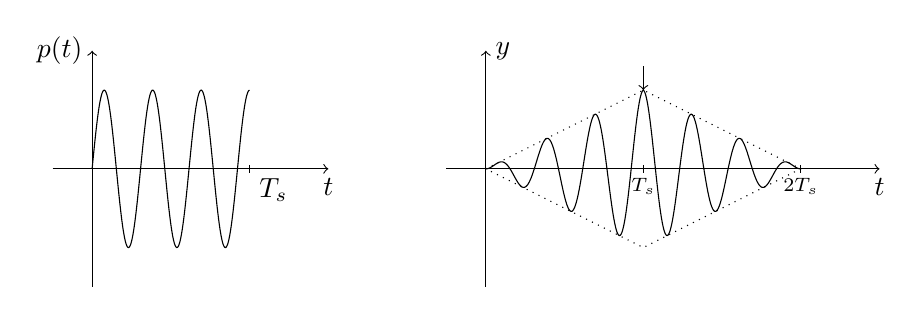
\begin{tikzpicture}
            \draw [->] (-0.5,0) -- (3,0) node [anchor=north] {$t$};
            \draw [->] (0,-1.5) -- (0,1.5) node [anchor=east] {$p(t)$};
            \draw [samples=200,domain=0:2] plot (\x,{sin(3.25*pi*\x r)});
            \draw (2,0.05) -- (2,-0.05);
            \path (2,0) node [below right=0mm] {$T_s$};
            \begin{scope}[shift={(5,0)}]
                \draw [->] (-0.5,0) -- (5,0) node [anchor=north] {$t$};
                \draw [->] (0,-1.5) -- (0,1.5) node [anchor=west] {$y$};
                \draw [samples=200,domain=0:2] plot (\x,{1/2*\x*sin(3.25*pi*\x r)});
                \draw [samples=200,domain=2:4] plot (\x,{1/2*(4-\x)*sin(3.25*pi*\x r)});
                \draw (2,0.05) -- (2,-0.05);
                \path (2,0) node[anchor=north] {$\scriptstyle T_s$};
                \draw (4,0.05) -- (4,-0.05);
                \path (4,0) node[anchor=north] {$\scriptstyle 2T_s$};
                \draw [dotted] (0,0) -- (2,1) -- (4,0) -- (2,-1) -- (0,0);
                \draw [->] (2,1.3) -- (2,1);
            \end{scope}
        \end{tikzpicture}
        \endpgfgraphicnamed\end{minipage}
    \end{figure}
    \FloatBarrier
\end{ejemplo}

La figura muestra la oscilación de la señal a muestrear, en
realidad es mucho más rápido que lo dibujado. Un error mínimo de
sincronización produciría un error. A continuación veremos una
alternativa que evita este problema y es equivalente si $f_c=n
f_s$.

\newpage

\subsection*{Detector coherente}


\begin{figure}[htb]
    \centering
    \resizebox{\textwidth}{!}{
    \bpgf{Imagenes/DDPasa/DDPasa-3}
    \begin{blockdiagram}
        \matrix[row sep=5 mm, column sep=10mm, ampersand replacement=\&]{
            \& \& \& \& \& \& \node[punto] (p1) {}; \& \node[etiqueta] (muestreo) {};\\
            \node [punto] (p6) {}; \& \& \node[operator] (mult) {$\times$}; \& \node [block] (filtro) {$\hat{H}(f)$}; \& \node [punto] (p2) {}; \&\node [punto] (p3) {}; \& \&\node [punto] (p4) {}; \&\node [block] (comp) {COMP};\\
            \& \& \node [etiqueta] (osc) {$2\cos(\omega_ct)$} node [below=3.5mm]{\parbox{3cm}{\centering }};
            \& \node [etiqueta] (ap) {\parbox{2cm}{\centering filtro apareado a $p(t)$}}; \& \& \node [block] (sinc) {SINCR}; \& \node [punto] (p5) {};\\
        };
        \draw [->] (p6) -- node [anchor=south east] {$\sum_k a_kp(t)\cos(\omega_ct)+n(t)$} (mult);
        \draw [->] (mult) -- (filtro);
        \draw [->] (osc) -- (mult);
        \draw [->,dotted] (ap) -- (filtro);
        \draw (filtro) -- (p2) -- node [anchor=south] {$y$} (p3) -- (muestreo);
        \draw [->] (p2) |- (sinc);
        \draw (sinc) -- (p5);
        \draw [->,dashed] (p5) -- (p1);
        \draw [->] (p4) -- (comp);
    \end{blockdiagram}
    \endpgfgraphicnamed}
\end{figure}
\FloatBarrier

Esencialmente, consiste en una demodulación sincrónica de la señal
DSB, combinada con una detección óptima de banda base.

\noindent {\bf Notas:}
%\begin{remarksSN}$\phantom{1}$
    \begin{itemize}
        \item El filtro acoplado de banda base también elimina la
        frecuencia doble $2f_c$.
        \item Colocamos una ganancia $2$ en el oscilador local. Esto simplifica las expresiones evitando el factor $\frac{1}{2}$ que aparec\'ia en la detección
        sincrónica analógica.
        Otra forma de motivarlo es observar que
        $||\tilde{p}||^2=\frac{1}{2}||p||^2$, y $K$ en el filtro
        acoplado se toma inversamente proporcional a esta
        cantidad.
        \item No require sincronismo fino en el muestreo, pero sí del oscilador local con la onda, por eso se llama \emph{detección coherente}.
            Es más fácil sincronizar osciladores que el muestreo.
        \item En la práctica, también se colocaría un pasabanda ``ancho'' de RF para limitar el ruido antes de la demodulación
        sincrónica; es decir que $n(t)$ es un ruido pasabanda de ancho $\gg$ que la banda de $x_c(t)$, ver después.
    \end{itemize}
%\end{remarksSN}

\begin{ejemplo}pulso NRZ
    \begin{center}\begin{minipage}{\textwidth}
        \bpgf{Imagenes/DDPasa/DDPasa-4}
        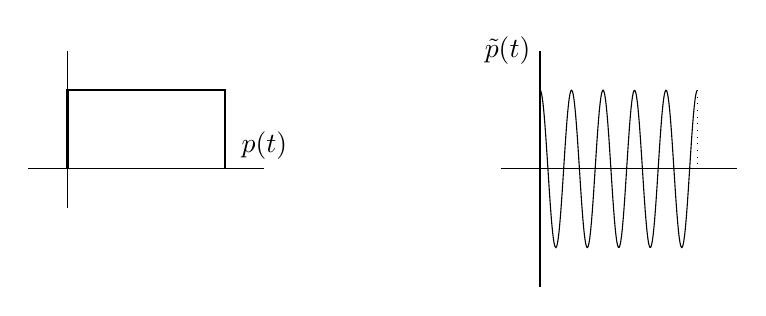
\begin{tikzpicture}
            \draw (-0.5,0) -- (2.5,0) node [anchor=south] {$p(t)$};
            \draw (0,-0.5) -- (0,1.5);
            \draw [thick] (0,0) -- (0,1) -- (2,1) -- (2,0);
            \begin{scope}[shift={(6,0)}]
                \draw (-0.5,0) -- (2.5,0);
                \draw (0,-1.5) -- (0,1.5) node [anchor=east] {$\tilde{p}(t)$};
                \draw [domain=0:2,samples=200] plot (\x,{cos(5*pi*\x r)});
                \draw [dotted] (2,1) -- (2,0);
            \end{scope}
        \end{tikzpicture}
        \endpgfgraphicnamed\end{minipage}
    \end{center}
    \begin{figure}[htb]
        \centering
        \resizebox{\textwidth}{!}{
        \bpgf{Imagenes/DDPasa/DDPasa-5}
            \begin{blockdiagram}[decoration={brace,amplitude=10}]
                \matrix[row sep=5 mm, column sep=10mm, ampersand replacement=\&]{
                    \& \& \& \& \& \node[punto] (p1) {}; \& \node[etiqueta] (muestreo) {};\\
                    \node [etiqueta] (p6) {$\sum_k a_k p(t)\cos(\omega_ct)+n(t)$}; \& \node[operator] (mult) {$\times$}; \& \node [block] (filtro) {$\displaystyle \frac{1}{T_s} \int_{t-T_s}^t$}; \& \node [punto] (p2) {}; \&\node [punto] (p3) {}; \& \&\node [punto] (p4) {}; \&\node [block] (comp) {COMP};\\
                    \& \node [etiqueta] (osc) {$2\cos(\omega_ct)$}; \& \& \& \node [block] (sinc) {SINCR}; \& \node [punto] (p5) {};\\
                };
                \draw [->] (p6) --  (mult);
                \draw [->] (mult) -- node [anchor=south] {$x_o(t)$} (filtro);
                \draw [->] (osc) -- (mult);
                %\draw (filtro) -- (p2) -- (p3) -- (muestreo);
                \draw (filtro) -- (p2) -- node [anchor=south] {$y$} (p3) -- (muestreo);
                \draw [->] (p2) |- (sinc);
                \draw (sinc) -- (p5);
                \draw [->,dashed] (p5) -- (p1);
                \draw [->] (p4) -- (comp);
                \draw [decorate]  (filtro.south east) --node [below=3mm] {\parbox{3cm}{filtro acop. a NRZ, integra en un período de símb.}} (filtro.south west);
            \end{blockdiagram}
            \endpgfgraphicnamed}
    \end{figure}
    \FloatBarrier
\end{ejemplo}
Analizamos este caso (pulso NRZ) de aquí en adelante por simplicidad.

\newpage

\noindent {\bf Notas:}
    \begin{itemize}
        \item Los pulsos rectangulares son los de uso más frecuente en radiofrecuencia, ya que es
             difícil hacer amplificadores de potencia para antena, que operen en forma lineal, lo que haría falta para pulsos de amplitud variable.
        \item Los pulsos de Nyquist se utilizan, por ejemplo, en TV cable digital.
    \end{itemize}



\subsection*{Análisis de probabilidad de error en el detector coherente con pulso NRZ}

Suponemos que el canal tiene ruido blanco Gaussiano, al que se
aplica un filtro pasabanda de entrada, centrado en $f_c$ y de
ancho mucho mayor que $f_s$, de modo de no distorsionar los
pulsos. El ruido recibido $n(t)$ tendrá densidad espectral de
potencia como se indica:

\begin{center}\begin{minipage}{\textwidth}
    \bpgf{Imagenes/DDPasa/DDPasa-6}
    \begin{tikzpicture}
        \draw [->] (-6,0) -- (6,0) node [anchor=north] {$f$};
        \draw [->] (0,-0.5) -- (0,1.5) node [anchor=east] {$S_n(f)$};
        \draw (-4,0) -- (-4,1) -- (-2,1) -- (-2,0) -- (2,0) -- (2,1) -- (4,1) node [anchor=west] {$\frac{\eta}{2}$} -- (4,0);
        \draw [dotted] (3,1) -- (3,0) node [anchor=north] {$f_c$};
    \end{tikzpicture}
    \endpgfgraphicnamed\end{minipage}
\end{center}

Modelamos el ruido pasabanda como
\[n(t) = n_i(t)\cos(\omega_ct) - n_q(t)\sen(\omega_ct),\]
donde $n_i$, $n_q$ son ruidos de banda base: $S_{n_i}=S_{n_q} =
\eta$ en una banda $[-B,B]$, $B \gg f_s$.

La señal de entrada es
\begin{align*}
    x_c(t)+n(t) &= \sum_k a_k p(t-kT_s)\cos(\omega_ct) + n_i(t)\cos(\omega_ct) - n_q(t)\sen(\omega_ct)\\
    \Rightarrow x_o(t) &= 2 [x_c(t)+n(t)]\cos(\omega_ct) = \sum_k a_k p(t-kT_s) + n_i(t) + \text{ términos de
    alta frecuencia.}
\end{align*}

Las componentes de alta frecuencia las elimina el filtro, por lo
que el problema se reduce a uno de detección óptima en banda base,
con ruido $n_i$. Esto  motiva colocar $h=\frac{1}{T_s}
p_{[0,T_s]}(t)$, el filtro acoplado al pulso NRZ. Obtenemos
\[y((k+1)T_s) = a_k \underbrace{(h\ast p)((k+1)T_s)}_{=1} + \underbrace{(h\ast n_i)((k+1)T_s)}_{n_k}.\]
\begin{center}
    \col{y_k=a_k+n_k}
\end{center}
La varianza del ruido es
\[\sigma^2=E[n_k^2] = E[n^2] = \int_{-\infty}^{+\infty}|\hat{H}(f)|^2\underbrace{S_{n_i}(f)}_{\eta}\d f \approx \eta ||h||^2 = \eta\frac{1}{T_s} = \eta f_s.\]

La hipótesis $B\gg f_s$ se utilizó en la aproximación de arriba. % En
%otras palabras: si el pasabanda de entrada es ancho como para
%dejar intacto el pulso, su equivalente pasabajos deja pasar toda
%la energía del filtro acoplado.
 O sea que tengo el mismo problema
de detección de banda base, polar o unipolar, con el doble de
ruido: $\sigma^2=\eta f_s$.

%Calculamos las correspondientes probabilidades de error \'optimas:


\begin{description}
    \item[ASK] $a_k=\{0,A\}$ (unipolar). Umbral: $\frac{A}{2}$,
    $P_e=Q\left(\frac{A}{2\sigma}\right)$.
    \item[BPSK] $a_k=\pm A$ (polar). Umbral: $0$,
    $P_e=Q\left(\frac{A}{\sigma}\right)$.
 \end{description}

Al igual que en banda base, se estila escribir $P_e$ en términos de
$\frac{\overline{E_p}}{\eta}$, donde $\overline{E_p} =
E[a_k^2]||\tilde{p}||^2$, energía media del pulso de RF
transmitido. \\ Aquí $\tilde{p}(t) = p(t)\cos(\omega_c t)
\Longrightarrow ||\tilde{p}||^2=\frac{1}{2}||p||^2=\frac{T_s}{2}$
para NRZ.

\begin{description}
    \item[ASK]
    \begin{equation*}
%        \left \lbrace
       \left. \begin{aligned} \overline{E_p}=\frac{A^2}{2}\frac{T_s}{2} \Rightarrow  A^2&=4 \overline{E_p} f_s\\
                                                            \sigma^2 &= \eta f_s
                                                           \end{aligned}\right\rbrace \Rightarrow
                                                           \frac{A}{2\sigma}=\sqrt{\frac{\overline{E_p}}{\eta}}.
    \end{equation*}
    \begin{center}
        \col{P_e=Q\left(\sqrt{\frac{\overline{E_p}}{\eta}}\right)} \  \ igual que en banda base unipolar.
    \end{center}

    \item[BPSK]
    \begin{equation*}
         \left.\begin{aligned}
          \overline{E_p}=A^2\frac{T_s}{2} \Rightarrow A^2 &=2 \overline{E_p} f_s\\
                                                            \sigma^2 &= \eta f_s
                                                           \end{aligned}\right\rbrace \Rightarrow
                                                           \frac{A}{\sigma}=\sqrt{2\frac{\overline{E_p}}{\eta}}.
    \end{equation*}
        \begin{center}
        \col{P_e=Q\left(\sqrt{2 \frac{\overline{E_p}}{\eta}}\right)} \  \ igual que en banda base polar.
    \end{center}
 \end{description}

A continuaci\'on, generalizamos el detector coherente y el an\'alisis de probabilidad de error para
las modulaciones pasabanda M-arias.

\newpage
\subsection*{Detección 4-QAM coherente}

Luego de un filtrado (de banda ancha) en la entrada, la señal que ingresa al detector es
\[
x_c(t)+ n(t) = \sum_k p(t-kT_s)\left[a_k\cos(\omega_ct)-b_k\sen(\omega_ct)\right] +
n(t),\]
donde $a_k=\pm A$, $b_k=\pm A$
independientes y equiprobables, y  el ruido es Gaussiano de densidad espectral de
potencia $\frac{\eta}{2}$ en la banda de inter\'es.

\subsubsection*{Detector coherente (para pulsos NRZ)}

\begin{figure}[htb]
    \centering
    \resizebox{\textwidth}{!}{
    \bpgf{Imagenes/DDPasa/DDPasa-7}
    \begin{blockdiagram}
        \matrix[row sep=5 mm, column sep=10mm, ampersand replacement=\&]{
            \& \& \& \& \& \& \node[punto] (p1) {}; \& \node[etiqueta] (muestreo) {};\\
            \node [punto] (inicio) {}; \& \node [punto] (p6) {}; \& \node[operator] (mult) {$\times$}; \& \node [block] (filtro) {$\displaystyle \frac{1}{T_s} \int_{t-T_s}^t$}; \& \node [punto] (p2) {}node [anchor=south] {$y$}; \&\node [punto] (p3) {}; \& \&\node [punto] (p4) {}; \&\node [block] (comp) {COMP}; \& \node [etiqueta] (salida) {$\hat{a}_k$};\\
            \& \& \node [etiqueta] (osc) {$2\cos(\omega_ct)$}; \& \& \& \node [block] (sinc) {SINCR}; \& \node [punto] (p5) {};\\
            \& \& \& \& \& \& \node[punto] (p1b) {}; \& \node[etiqueta] (muestreob) {};\\
            \& \& \node[operator] (multb) {$\times$}; \& \node [block] (filtrob) {$\displaystyle \frac{1}{T_s} \int_{t-T_s}^t$}; \& \node [punto] (p2b) {} node [anchor=south] {$z$}; \&\node [punto] (p3b) {}; \& \&\node [punto] (p4b) {}; \&\node [block] (compb) {COMP}; \& \node [etiqueta] (salidab) {$\hat{b}_k$};\\
            \& \& \node [etiqueta] (oscb) {$-2\sen(\omega_ct)$}; \& \& \& \node [block] (sincb) {SINCR}; \& \node [punto] (p5b) {};\\
        };
        \draw (inicio) -- (p6);
        \draw [->] (p6) --  (mult);
        \draw [->] (mult) -- (filtro);
        \draw [->] (osc) -- (mult);
        \draw (filtro) -- (p2) -- (p3) -- (muestreo);
        \draw [->] (p2) |- (sinc);
        \draw (sinc) -- (p5);
        \draw [->,dashed] (p5) -- (p1);
        \draw [->] (p4) -- (comp);
        \draw [->] (comp) -- (salida);

        \draw [->] (p6) |-  (multb);
        \draw [->] (multb) -- (filtrob);
        \draw [->] (oscb) -- (multb);
        \draw (filtrob) -- (p2b) -- (p3b) -- (muestreob);
        \draw [->] (p2b) |- (sincb);
        \draw (sincb) -- (p5b);
        \draw [->,dashed] (p5b) -- (p1b);
        \draw [->] (p4b) -- (compb);
        \draw [->] (compb) -- (salidab);
    \end{blockdiagram}
    \endpgfgraphicnamed}
\end{figure}

Similar al detector QAM analógico, aquí el filtro es el acoplado.

Escribimos el ruido como $n_i(t)\cos(\omega_ct)-n_q(t)\sen(\omega_ct)$, tenemos
\begin{align*}
    y((k+1)T_s) &= a_k + (h\ast n_i)((k+1)T_s) = a_k + n_k^i,\\
    z((k+1)T_s) &= b_k + (h\ast n_q)((k+1)T_s) = b_k + n_k^q,\\
\end{align*}
donde $n_k^i, n_k^q$ son Gaussianos $(0,\sigma^2=\eta f_s)$ (igual
que en BPSK). Suponiendo que el filtro de entrada es simétrico
alrededor de $f_c$, $n_i(t)$ y $n_q(t)$ son no correlacionados y
luego (por ser Gaussianos) son independientes. Por tanto $n_k^i,
n_k^q$ son variables aleatorias independientes.

Las probabilidades de error en la detección de cada $a_k$ y $b_k$
son
\[P_e(a_k) = P_e(b_k) = Q\left(\frac{A}{\sigma}\right).\]
La probabilidad de error de símbolo es
\[
P_e(\text{simb})= 1 - (1-P_e(a_k))(1-P_e(b_k)) \approx 2
Q\left(\frac{A}{\sigma}\right).\]

\subsubsection*{Expresión con $\frac{\overline{E_p}}{\eta}$}

\begin{gather*}
    \overline{E_p}=\underbrace{E[a_k^2]}_{A^2} \underbrace{\left\|p(t)\cos(\omega_ct)\right\|^2}_{\frac{T_s}{2}} + \underbrace{E[b_k^2]}_{A^2} \underbrace{\left\|p(t)\sen(\omega_ct)\right\|^2}_{\frac{T_s}{2}} = A^2 T_s\\
    \Rightarrow \frac{A}{\sigma}=\sqrt{\frac{\overline{E_p}}{\eta}}
    \Rightarrow  P_e(\text{simb})  = 2
    Q\left(\sqrt{\frac{\overline{E_p}}{\eta}}\right).
\end{gather*}

Para comparar correctamente con las modulaciones binarias,
conviene considerar la probabilidad de error de bit
\[
P_e(\text{bit})=Q\left(\frac{A}{\sigma}\right),\] y tambi\'en
introducir la \emph{energ\'ia media por bit}, que considera que
cada pulso lleva 2 bits:
\[
\overline{E_b} = \frac{1}{2}\overline{E_p}.
\]
Se obtiene entonces (igual que en BPSK) la expresi\'on
\[
P_e(\text{bit}) = Q\left(\sqrt{\frac{2
\overline{E_b}}{\eta}}\right).
\]


\subsection*{Generalización: QAM M-ario}

\noindent Suponemos $M=M_a^2=M_b^2$, y usamos los niveles $\pm
A,\pm 3A,\ldots,\pm(\sqrt{M}-1)A$ para $a_k$ y $b_k$


En el intervalo $[k T_s, (k+1)T_s]$, la onda enviada
$\left[a_k\cos(\omega_ct)-b_k\sen(\omega_ct)\right]$ es sinusoidal con envolvente compleja (fasor) $(a_k+jb_k)$, punto de la constelación.
En ausencia de ruido, la correlaci\'on con las componentes $\cos(\omega_ct)$ y $\sen(\omega_ct)$ producir\'ia precisamente los s\'imbolos $a_k$, $b_k$. El efecto del ruido es ``borronear" los puntos de la constelaci\'on. La tarea del detector es clasificar cual fue el punto enviado, lo que se hace mediante umbrales en las componentes en fase y cuadratura.

El detector es igual al 4QAM, excepto que cada variable $y_k$, $z_k$ se compara con más umbrales.


\newpage

%
%    \begin{figure}[htb]
%        \centering
\begin{minipage}{0.5\textwidth}
\begin{ejemplo} 16 QAM, $\sqrt{M}=4$
\begin{itemize}
    \item $y_k$ es cuaternario $\rightarrow$ umbrales $0,\pm 2A$.
    \item $z_k$ es cuaternario $\rightarrow$ umbrales $0,\pm 2A$.
\end{itemize}
\end{ejemplo}
\end{minipage}
\begin{minipage}{0.5\textwidth}
    \resizebox{\textwidth}{!}{
        \bpgf{Imagenes/DDPasa/DDPasa-8}
        \begin{tikzpicture}
            \draw [->] (-4,0) -- (4,0);
            \draw [->] (0,-4) -- (0,4);
            \foreach \x in {-3,-1,...,3}
                {\draw  (\x,-3) -- (\x,3);
                \draw  (-3,\x) -- (3,\x);
                \foreach \y in {-3,-1,...,3}
                    \draw [fill] (\x,\y) circle (0.07);}
            \path (-3,0) node [anchor=north east] {$-3A$} -- (-1,0) node [anchor=north east] {$-A$} (1,0) node [anchor=north west] {$A$} -- (3,0) node [anchor=north west] {$3A$};
            \draw [dotted] (2,-3.5)  node [anchor=north west] {umbrales de detección}-- (2,3.5);
            \draw [dotted] (-2,-3.5) -- (-2,3.5);
            \draw [dotted] (-3.5,2) -- (3.5,2);
            \draw [dotted] (-3.5,-2) -- (3.5,-2);
        \end{tikzpicture}
        \endpgfgraphicnamed}\end{minipage}
%    \end{figure}
%    \FloatBarrier


Recordando la detecci\'on M-aria en banda base,
$P_e(a_k)=2\frac{M_a-1}{M_a} Q\left(\frac{A}{\sigma}\right)$.

Incluyendo $M_a=\sqrt{M}$, y considerando también $P_e(b_k)$
obtenemos

\[
P_e(\text{simb})=4\frac{\sqrt{M}-1}{\sqrt{M}}
Q\left(\frac{A}{\sigma}\right).\]

\paragraph{Expresión con $\overline{E_p}$}

\begin{gather*}
    \overline{E_p}=\left(E[a_k^2]+E[b_k^2]\right)\frac{T_s}{2} =  E[a_k^2]T_s = \frac{M_a^2-1}{3} A^2T_s = \frac{M-1}{3} A^2T_s  \\
    \Rightarrow A^2= \frac{3 \overline{E_p}}{M-1} f_s \Rightarrow \frac{A}{\sigma} = \sqrt{\frac{3\overline{E_p}}{(M-1)\eta}}.\\
    \col{P_e(\text{simb}) = 4\frac{\sqrt{M}-1}{\sqrt{M}}Q\left(\sqrt{\frac{3\overline{E_p}}{(M-1)\eta}}\right)}
\end{gather*}

%\newpage

\subsection*{Detección PSK M-aria}
%
%\begin{figure}[htb]
    \begin{center}
\begin{minipage}{0.4\textwidth}
    \resizebox{\textwidth}{!}{
    \bpgf{Imagenes/DDPasa/DDPasa-9}
    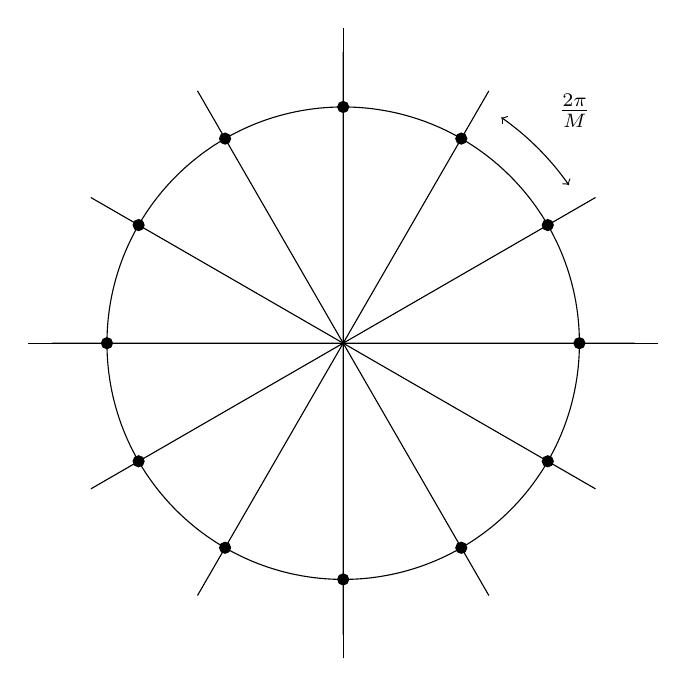
\begin{tikzpicture}
        \draw (-4,0) -- (4,0);
        \draw (0,-4) -- (0,4);
        \draw (0,0) circle (3);
        \foreach \x in {0,30,...,330}
            \draw [fill] (0,0) -- (\x:3) circle (0.07) -- (\x:3.7);
        \draw (35:3.5) [<->] arc (35:55:3.5);
        \path (45:3.7) node [anchor=south west] {$\frac{2\pi}{M}$};
    \end{tikzpicture}
    \endpgfgraphicnamed}
    \end{minipage}%
\end{center}
%\end{figure}
%\FloatBarrier

\begin{figure}[htb]
    \centering    \resizebox{\textwidth}{!}{
    \bpgf{Imagenes/DDPasa/DDPasa-10}
    \begin{blockdiagram}
        \matrix[row sep=5 mm, column sep=10mm, ampersand replacement=\&]{
            \& \& \& \& \& \node [punto] (p1a) {};\\
            \node [etiqueta] (inicio) {$Ap(t)\cos(\omega_ct+\theta_k)+n(t)$}; \& \node [punto] (p) {};\& \node[operator] (multa) {$\times$}; \& \node[block] (filtroa) {$\frac{1}{T}\int$}; \& \node[punto] (p2a) {}; \& \node [punto] (p3a) {}; \& \node[etiqueta] (salidaa) {$A\cos(\theta_k)+n_k^i$};\\
            \& \& \node[etiqueta] (osca) {$2\cos(\omega_ct)$};\\
            \& \& \& \& \& \node [punto] (p1b) {};\\
            \& \& \node[operator] (multb) {$\times$}; \& \node[block] (filtrob) {$\frac{1}{T}\int$}; \& \node[punto] (p2b) {}; \& \node [punto] (p3b) {}; \& \node[etiqueta] (salidab) {$A\sen(\theta_k)+n_k^q$};\\
            \& \& \node[etiqueta] (oscb) {$-2\sen(\omega_ct)$};\\
        };
        \draw (inicio) -- (p);
        \draw [->] (p) -- (multa);
        \draw [->] (osca) -- (multa);
        \draw [->] (multa) -- (filtroa);
        \draw (filtroa) -- (p2a) -- (p1a);
        \draw [->] (p3a) -- (salidaa);

        \draw [->] (p) |- (multb);
        \draw [->] (oscb) -- (multb);
        \draw [->] (multb) -- (filtrob);
        \draw (filtrob) -- (p2b) -- (p1b);
        \draw [->] (p3b) -- (salidab);
    \end{blockdiagram}
    \endpgfgraphicnamed}
\end{figure}
\FloatBarrier

Ruido $(n_k^i,n_k^q)$ igual que en QAM.

\begin{figure}[htb]
    \centering\begin{minipage}{\textwidth}
    \bpgf{Imagenes/DDPasa/DDPasa-11}
    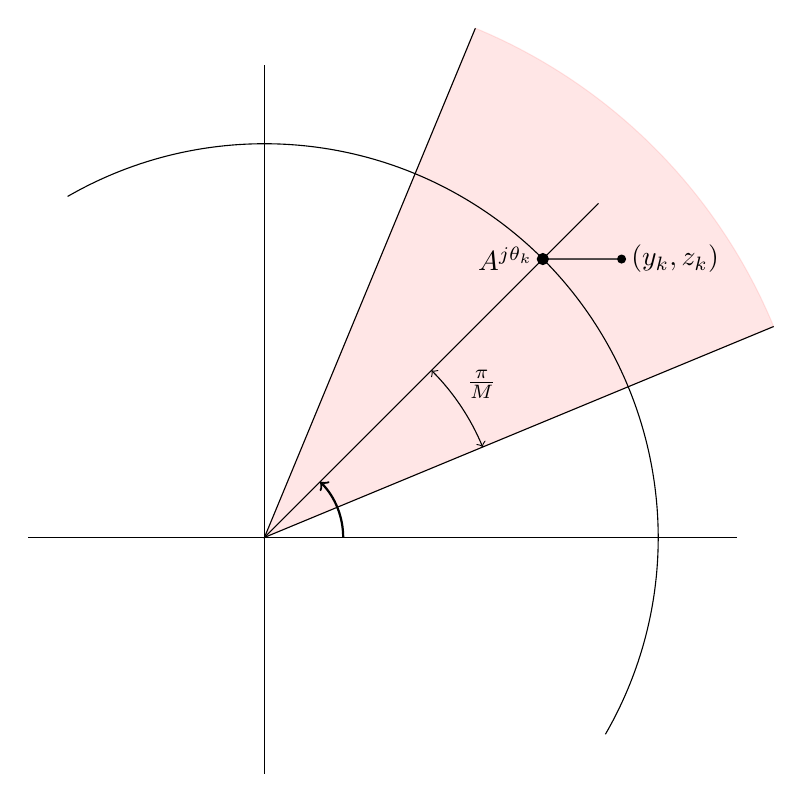
\begin{tikzpicture}
        \draw [fill,red!50,opacity=0.2] (0,0) -- (22.5:7)  arc (22.5:67.5:7) -- (0,0);
        \draw (-30:5) arc (-30:120:5);
        \draw (-3,0) -- (6,0);
        \draw (0,-3) -- (0,6);
        \draw (22.5:7) -- (0,0) -- (67.5:7);
        \draw (0,0) -- (45:6);
        \draw [->,thick] (1,0) arc (0:45:1);
        \draw [<->] (22.5:3)  arc  (22.5:45:3);
        \path (22.5:3) -- (45:3) node [anchor=south west,midway] {$\frac{\pi}{M}$};
        \draw [fill] (45:5) circle (0.07) node [anchor=east] {$A\e^{j\theta_k}$};
        \draw [fill] (45:5) -- ++(1,0) circle (0.05) node [anchor=west] {$(y_k,z_k)$};
    \end{tikzpicture}
    \endpgfgraphicnamed \end{minipage}
\end{figure}
\FloatBarrier

Umbrales de detección: al recibir $(y_k,z_k)$ busco el símbolo más
cercano $\Rightarrow$ umbrales radiales. La $P_e$ no depende del
símbolo enviado.



Para calcular $P_e$, por simplicidad tomo
$\theta_k=0$.

\begin{minipage}{0.5\textwidth}
    \resizebox{\textwidth}{!}{
%\begin{center}
    \bpgf{Imagenes/DDPasa/DDPasa-11b}
    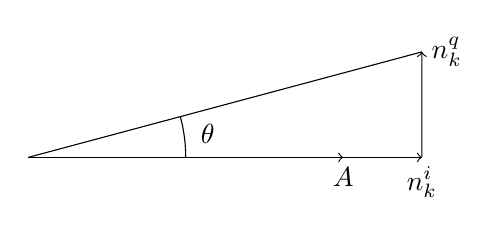
\begin{tikzpicture}
        \draw [->] (0,0) -- (4,0) node [anchor=north] {$A$};
        \draw [->] (4,0) -- (5,0) node [anchor=north] {$n^i_k$};
        \draw [->] (5,0) -- (intersection of 0,0--15:1 and 5,0--5,1) node [anchor=west] {$n^q_k$};
        \draw (0,0) -- (intersection of 0,0 -- 15:1 and 5,0--5,1);
        \draw (2,0) arc (0:15:2);
        \path (7.5:2.3) node {$\theta$};
    \end{tikzpicture}
    \endpgfgraphicnamed}
%\end{center}
\end{minipage}\hfil
\begin{minipage}{0.5\textwidth}
\begin{gather*}
    \tan(\theta)=\frac{n^q_k}{A+n^i_k},\\
    P_e(\text{simb}) = P\left(|\theta|>\frac{\pi}{M}\right).
\end{gather*}
\end{minipage}

Esto es complejo de evaluar analíticamente, pero existe una
aproximación para $M\geq 4$ y $A \gg \sigma$:
\[P_e(\text{simb})\approx 2 Q\left(\sqrt{\frac{\overline{E_p}}{\frac{\eta}{2}}\sen^2\left(\tfrac{\pi}{M}\right)}\right).\]


\subsection*{Comparación MQAM-MPSK(M grande)}

\begin{description}
    \item[QAM] $P_e\approx 4 Q\left(\sqrt{\frac{3\overline{E_p}}{M\eta}}\right)$
    \item[PSK] $P_e\approx 2 Q\left(\sqrt{\frac{2\pi^2\overline{E_p}}{M^2\eta}}\right)$.
 \end{description}
El argumento de la funci\'on $Q(\cdot)$ cae más rápido con $M$ en
PSK que en QAM
\\$\Longrightarrow P_e$ es mayor (peor) en PSK que en QAM.  \\

 {\bf QAM superior a MPSK (M
grande).}

\paragraph{Intuición: } La separación de los puntos de la constelación, en relación al ruido es lo que determina $P_e$.
La restricción de potencia (o $\overline{E_p}$) limita cuan lejos
en el plano se puede extender la constelación. Entonces, para
lograr la mejor $P_e$ con una $\overline{E_p}$ dada, lo mejor es
una constelación uniforme de puntos en el plano. Esto se consigue
mejor con QAM.

\begin{figure}[htb]
    \centering
    \resizebox{\textwidth}{!}{
    \bpgf{Imagenes/DDPasa/DDPasa-12}
    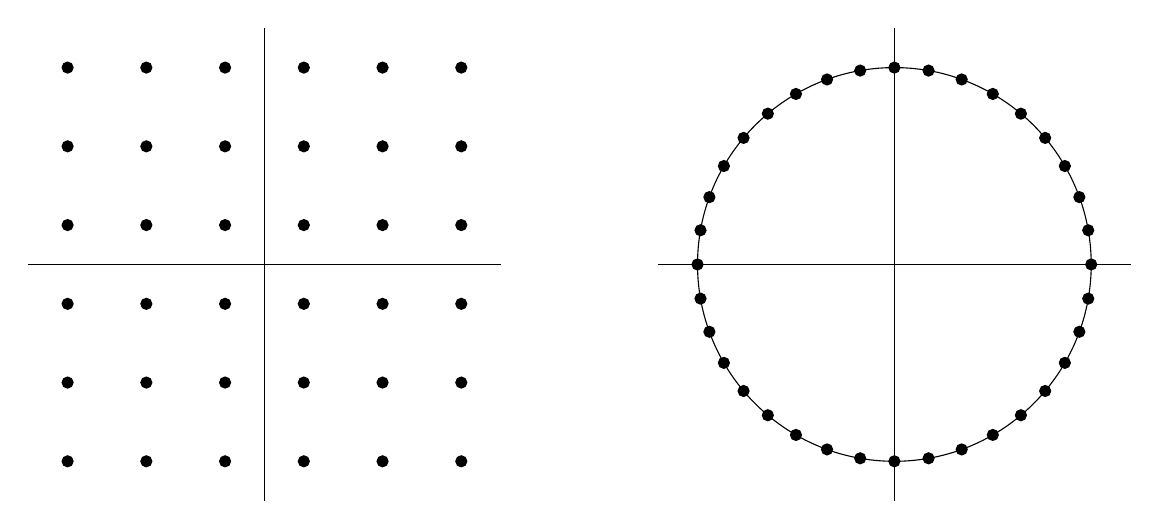
\begin{tikzpicture}
        \draw (-3,0) -- (3,0);
        \draw (0,-3) -- (0,3);
        \foreach \x in {-2.5,-1.5,...,2.5}
            \foreach \y in {-2.5,-1.5,...,2.5}
                \draw [fill] (\x,\y) circle (0.07);
        \begin{scope}[shift={(8,0)}]
            \draw (-3,0) -- (3,0);
            \draw (0,-3) -- (0,3);
            \draw (0,0) circle (2.5);
            \foreach \x in {0,10,...,350}
                \draw [fill] (\x:2.5) circle (0.07);
        \end{scope}
    \end{tikzpicture}
    \endpgfgraphicnamed}
\end{figure}
\FloatBarrier

Las anteriores son las probabilidades de error de símbolo. Igual
que en banda base, se plantea el tema de cuantos bits son
afectados por cada error de símbolo.

Claramente, son mucho más probables los errores a un vecino de la
constelación. Si logramos codificar los bits de modo que símbolos
vecinos difieran en un sólo bit (codificación de Gray), tenemos
que


\[P_e(\text{bit})=\text{``BER''} = \col{\frac{P_e(\text{simb})}{\log_2(M)}}\]

%\newpage
\subsubsection*{Coficaci\'on de Gray}

Para MPSK, la constelación es esencialmente unidimensional (en un
círculo), por lo tanto podemos generar codigos de Gray en forma
similar al caso de banda base. Ejemplo de 8-PSK:


\begin{figure}[htb]
    \centering\begin{minipage}{\textwidth}
    \bpgf{Imagenes/DDPasa/DDPasa-14}
    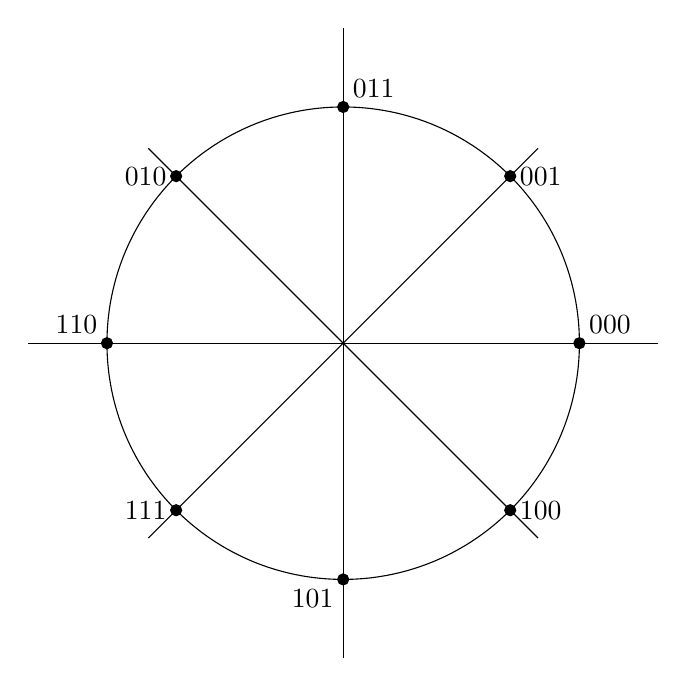
\begin{tikzpicture}
        \draw (-4,0) -- (4,0);
        \draw (0,-4) -- (0,4);
        \draw (0,0) circle (3);
        \foreach \x in {0,45,...,315}
            {\draw [fill] (\x:3) circle (0.07);
            \draw (0,0) -- (\x:3.5);}
        \path (0:3) node [anchor=south west] {$000$};
        \path (45:3) node [anchor=west] {$001$};
        \path (90:3) node [anchor=south west] {$011$};
        \path (135:3) node [anchor=east] {$010$};
        \path (180:3) node [anchor=south east] {$110$};
        \path (225:3) node [anchor=east] {$111$};
        \path (270:3) node [anchor=north east] {$101$};
        \path (315:3) node [anchor=west] {$100$};
    \end{tikzpicture}
    \endpgfgraphicnamed\end{minipage}
\end{figure}


Para lograr esta propiedad en QAM hace falta una codificación de
Gray para una constelación bidimensional. La solución es coficar
por Gray  cada coordenada, que representa bits independientes.
Ejemplo con 16-QAM:


    \FloatBarrier
    \begin{figure}[htb]
        \centering\begin{minipage}{\textwidth}
        \bpgf{Imagenes/DDPasa/DDPasa-13}
        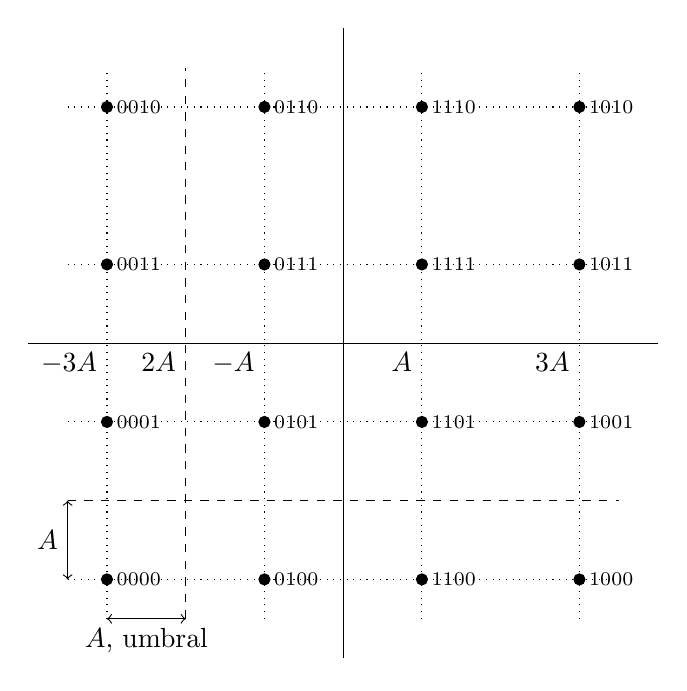
\begin{tikzpicture}
            \draw (-4,0) -- (4,0);
            \draw (0,-4) -- (0,4);
            \foreach \x/\p in {-3/-3,-1/-,1/{},3}
                {\draw [dotted] (\x,-3.5) -- (\x,3.5);
                \draw [dotted] (-3.5,\x) -- (3.5,\x);
                \path (\x,0) node  [anchor=north east] {$\p A$};
                \foreach \y in {-3,-1,...,3}
                    \draw [fill] (\x,\y) circle (0.07);}
            \path (-3,-3) node [anchor=west] {$\scriptstyle 0000$};
            \path (-1,-3) node [anchor=west] {$\scriptstyle 0100$};
            \path (1,-3) node [anchor=west] {$\scriptstyle 1100$};
            \path (3,-3) node [anchor=west] {$\scriptstyle 1000$};

            \path (-3,-1) node [anchor=west] {$\scriptstyle 0001$};
            \path (-1,-1) node [anchor=west] {$\scriptstyle 0101$};
            \path (1,-1) node [anchor=west] {$\scriptstyle 1101$};
            \path (3,-1) node [anchor=west] {$\scriptstyle 1001$};

            \path (-3,3) node [anchor=west] {$\scriptstyle 0010$};
            \path (-1,3) node [anchor=west] {$\scriptstyle 0110$};
            \path (1,3) node [anchor=west] {$\scriptstyle 1110$};
            \path (3,3) node [anchor=west] {$\scriptstyle 1010$};

            \path (-3,1) node [anchor=west] {$\scriptstyle 0011$};
            \path (-1,1) node [anchor=west] {$\scriptstyle 0111$};
            \path (1,1) node [anchor=west] {$\scriptstyle 1111$};
            \path (3,1) node [anchor=west] {$\scriptstyle 1011$};

            \draw [dashed] (-2,-3.5) -- (-2,3.5);
            \draw [dashed] (-3.5,-2) -- (3.5,-2);
            \path (-2,0) node [anchor=north east] {$2A$};
            \draw [<->] (-3.5,-2) -- node [anchor=east] {$A$} (-3.5,-3);
            \draw [<->] (-3,-3.5) -- node [anchor=north] {$A$, umbral} (-2,-3.5);
        \end{tikzpicture}
        \endpgfgraphicnamed\end{minipage}
    \end{figure}
    \FloatBarrier
Errores de más de $1$ bit requieren errores en dos coordenadas
(distancia $\sqrt{2}A$), o en una coordenada, pero más de un
salto.


\subsubsection*{Comparación (Carlson)}

Una forma de evaluar la eficiencia relativa de MQAM y MPSK con
codificación de Gray es definir
$E_b=\frac{\overline{E_p}}{\log_2(M)}$ (energía por bit) y
graficar la eficiencia espectral en función de $\frac{E_b}{\eta}$,
para una BER (probabilidad de error de bit) fija.

\begin{figure}[htb]
 \centering\begin{minipage}{\textwidth}
 \bpgf{Imagenes/DDPasa/DDPasa-14b}

  \begin{tikzpicture}
      \draw [->] (-0.5,0) -- (5,0) node [anchor=north] {$\frac{E_b}{\eta}$};
      \draw [->] (0,-0.5) -- (0,6) node [anchor=east] {$\frac{bps}{Hz}$};
      \draw [dotted] (0,1) node [anchor=east] {$2$} -- (1,1) -- (1,2) [dotted] -- (0,2) node [anchor=east] {$4$};
      \draw (1,1) -- (1,2);
      \draw (1,2) -- (4.5,5) node [anchor=west] {PSK};
      \draw (0,4) -- (5,4);
      \path ({10/3},4) node [anchor=north] {$16$};
      \draw [domain=1:4.5] plot (\x,{2.5*ln(\x)+2}) node [anchor=west] {QAM};
      \path ({exp(2/2.5)},4) node [anchor=south] {$16$};
  \end{tikzpicture}
  \endpgfgraphicnamed\end{minipage}

\end{figure}

